\documentclass[10pt,a4paper,oneside,fleqn]{report}
\usepackage{geometry}
\geometry{a4paper,left=20mm,right=20mm,top=1cm,bottom=2cm}
\usepackage[utf8]{inputenc}
%\usepackage{ngerman}
\usepackage{amsmath}                % brauche ich um dir Formel zu umrahmen.
\usepackage{amsfonts}                % brauche ich für die Mengensymbole
\usepackage{graphicx}
\setlength{\parindent}{0px}
\setlength{\mathindent}{10mm}
\usepackage{bbold}                    %brauche ich für die doppel Zahlen Darstellung (Einheitsmatrix z.B)
\usepackage[linktocpage={false}]{hyperref}


\usepackage{color}
\usepackage{titlesec} %sudo apt-get install texlive-latex-extra

\definecolor{darkblue}{rgb}{0.1,0.1,0.55}
\definecolor{darkred}{rgb}{0.55,0.2,0.2}

\titleformat{\chapter}[display]{\color{darkred}\normalfont\huge\bfseries}{\chaptertitlename\
\thechapter}{20pt}{\Huge}

\titleformat{\section}{\color{darkblue}\normalfont\Large\bfseries}{\thesection}{1em}{}
\titleformat{\subsection}{\color{darkblue}\normalfont\Large\bfseries}{\thesection}{1em}{}

% Notiz Box
\usepackage{fancybox}
\newcommand{\notiz}[1]{\vspace{5mm}\ovalbox{\begin{minipage}{1\textwidth}#1\end{minipage}}\vspace{5mm}}

\usepackage{cancel}



%\includegraphics[width=0.75\textwidth]{thepic.png}
%couchdb db=physik
%couchdb id=festkvorles06_Gitterdynamik_und_Phononen
%couchdb tags=festk
%couchdb pdflink=http://wernwa-physik-ka.googlecode.com/svn/festk/kap06.pdf

\begin{document}
\tableofcontents
\setcounter{chapter}{5}
\chapter{Gitterdynamik und Phononen}

\section{Gitterschwingungen}

1D Kette mit einatomiger Basis. 

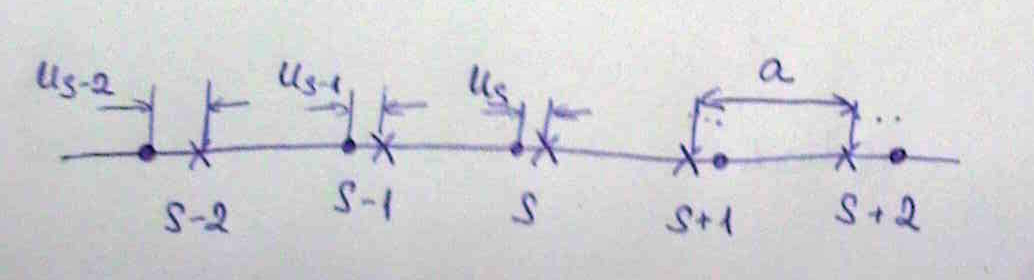
\includegraphics[width=0.75\textwidth]{kap06_01.png}

Bewegungsgleichungen:

\[ M\frac{d^2 u_s}{dt^2} = \sum^{\infty}_{n=-\infty}c_n(u_{s+n}-u_s)\]
mit \(c_n\) als Kraftkonstante

Lösung: \(u_{s+n}=v e^{-i\omega t + igna}\)

\[\omega^2 M = \sum^{\infty}_{n=-\infty}c_n(1-e^{iqna})\]

nach Symmetrie \(c_{-n}=c_n\)

\[\omega^2 = \frac{1}{M} \sum^{\infty}_{n=-\infty}c_n(2-e^{iqna}-e^{-iqna})=\frac{2}{M} \sum^{\infty}_{n=-\infty}c_n(2-cos(qna))\]
\(c_1 >> c_n\), für  \(n\geq 2\), nur nächst. Nachbarn \(\rightarrow \omega^2=\frac{2c_1}{M} (1-cos(qa)) =\frac{4c_1}{M} (sin^2(\frac{qa}{2}))\)

\[\omega = 2\sqrt{\frac{c_1}{M}}\left| sin\frac{qa}{2}\right|\]

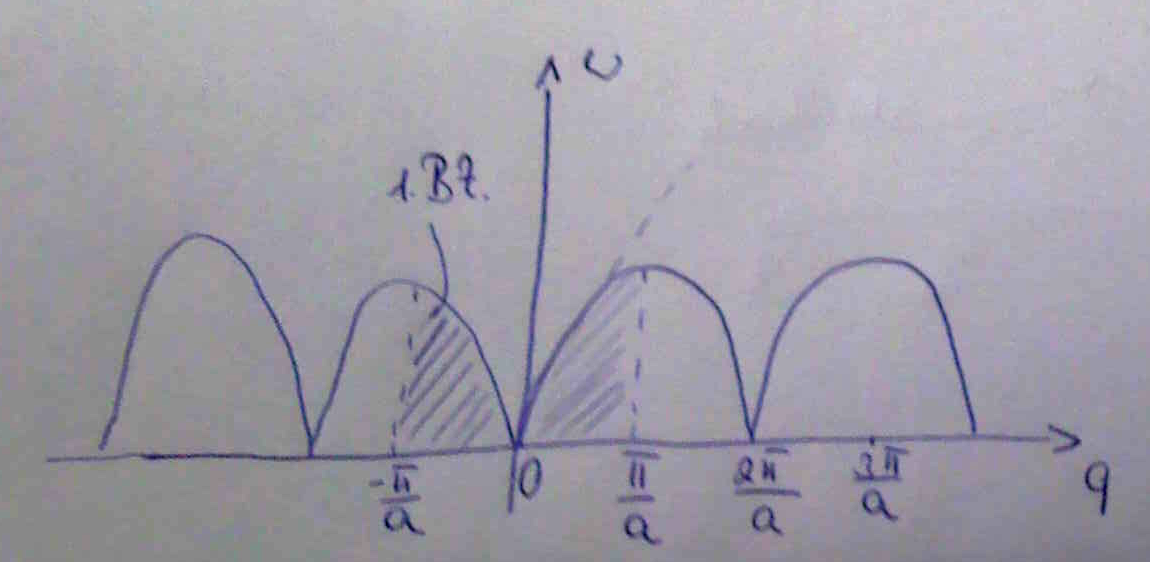
\includegraphics[width=0.75\textwidth]{kap06_02.png}

bei \(c_2\neq 0\); \(\omega^2 = \frac{4c_1}{M}\left[\ sin^2\frac{qa}{2} + \frac{c_2}{c_1}sin^2(qa) \right]\)

\(\frac{u_{s+1}}{u_s} = e^{iqa}\rightarrow\) Phasenunterschied

Wir betrachten den Bereich \(-\pi < qa < \pi\). Reduktion auf die 1. Brillouin-Zone; \(\underbrace{q'}_{\text{außerhalb 1 BZ}}=\underbrace{q}_{\text{1 BZ}}+\frac{2\pi N}{a}\) mit \(N\in \mathbb Z\)

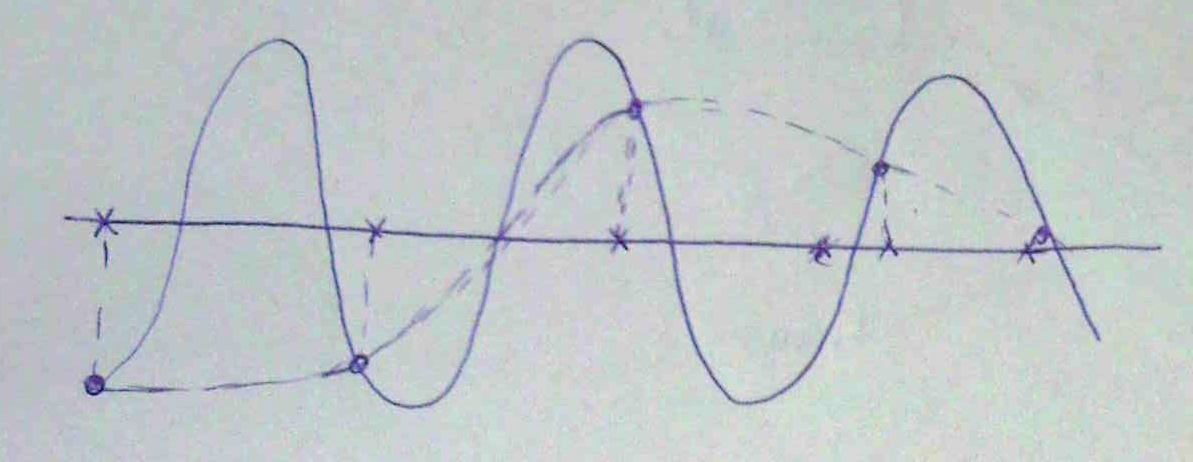
\includegraphics[width=0.75\textwidth]{kap06_03.png}

\(\frac{u_{s+1}}{u_s} = e^{iqa}\cdot e^{2\pi N}\)

- Gruppengeschwindigkeit: \(v_g = \frac{d\omega}{dq}\) (entspricht den Energietransport) (\(v_g=0\) eine Stehende Welle, Schwinung in Gegenphase, kein Energietransport)
- Phasengeschwindigkeit: \(v_{Ph} = \frac{\omega}{q}\)

Langwelliger Grenzfall: \(q\rightarrow 0\); \(\lambda \rightarrow \infty\)

\[\omega^2 = \frac{2}{M} \sum^{\infty}_{n=1}c_n(1-\underbrace{cos(qna)}_{\approx 1-\frac{x^2}{2}+...})\approx \frac{q^2a^2}{M}\sum^{\infty}_{n=1}n^2s_n\]
\[ c_{11} = \sum^{\infty}_{n=1} \frac{n^2}{a}c^2_n\]

kurzwelliger Grenzfall: \(|q|\approx \frac{\pi}{a}\); \(\lambda = 2a\)

 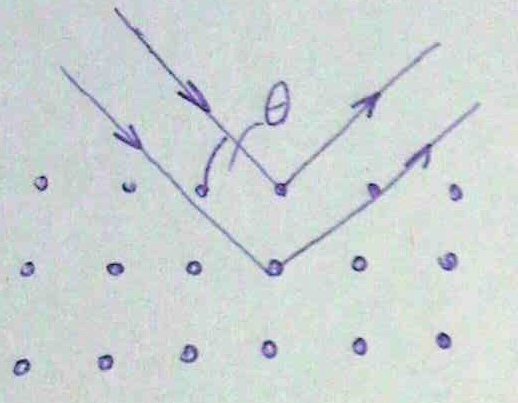
\includegraphics[width=0.75\textwidth]{kap06_04.png}

\(2dsin\theta=\lambda\); \(d=a\); \(\theta = \frac{\pi}{2}\)

\section{Gitter mit 2-Atomiger Basis}

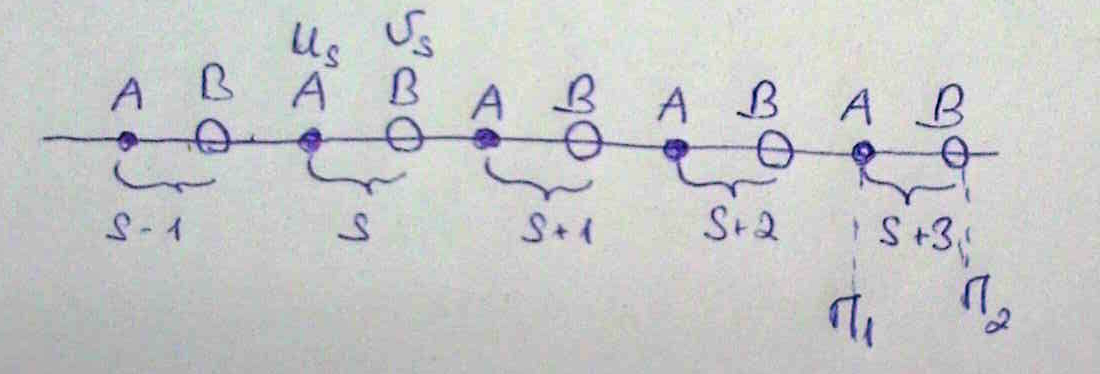
\includegraphics[width=0.75\textwidth]{kap06_05.png}

\[ M_1\frac{d^2 u_s}{dt^2} = c'(v_s-u_s)-c''(u_s-v_{s-1})\]
\[ M_2\frac{d^2 u_s}{dt^2} = c''(v_{s+1}-v_s)-c'(v_s-u_s)\]

Lösung \(u_s=ue^{-i\omega t + iqsa}\); \(v_s=ve^{-i\omega t + iqsa}\)



\(det|...|=0\); Eigenfrequenzen: \(\omega^2_{\pm} = \frac{\omega^2_0}{2}\left[1\pm \sqrt{1-\gamma^2 sin^2\frac{qa}{2}} \right]\)


\(\gamma = e \frac{\sqrt{c'c''}}{c'+c''}\cdot \frac{\sqrt{M'_1 M'_2}}{M_1+M_2}\); \(\omega_0 = (c'+c'')(\frac{1}{M_1}+\frac{1}{M_2})\)

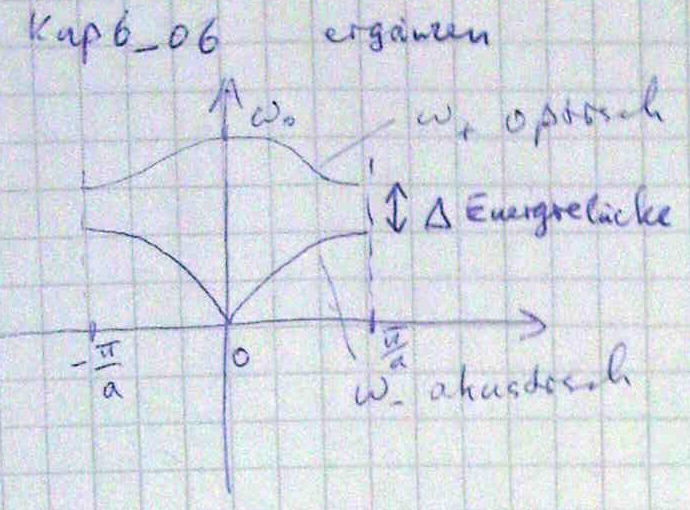
\includegraphics[width=0.75\textwidth]{kap06_06.png}


a) Für \(q\rightarrow 0\); \(\omega_0=\frac{2C}{\mu}\); \(c=c'=c''\); \(\mu^{-1}=\mu^{-1}_1+\mu^{-1}_2\)

\(\frac{u}{v}= -\frac{\mu_2}{\mu_1}\): Schwinung in Gegenphase; Ionenkristalle: oszillierendes elektrisches Dipolmoment

b) Für \(|q|\rightarrow \frac{\pi}{a}\); \(M_1<M_2\); \(\omega^2=\frac{2c}{M_1}\); \(\omega^2=\frac{2c}{M_2}\) \(\Rightarrow \frac{v}{u}=0\) bzw \(\frac{u}{v}=0\)

Frequenzlücke \(\rightarrow\) 'verbotene' Zone

\underline{3D Kristalle (mit P Atomen pro E.Z.)}

\begin{itemize}
\item Es gibt 3 akustische Zweige mit 1 longitudinale und 2 transversale
\item (3P-3) optische Zweige
\end{itemize}

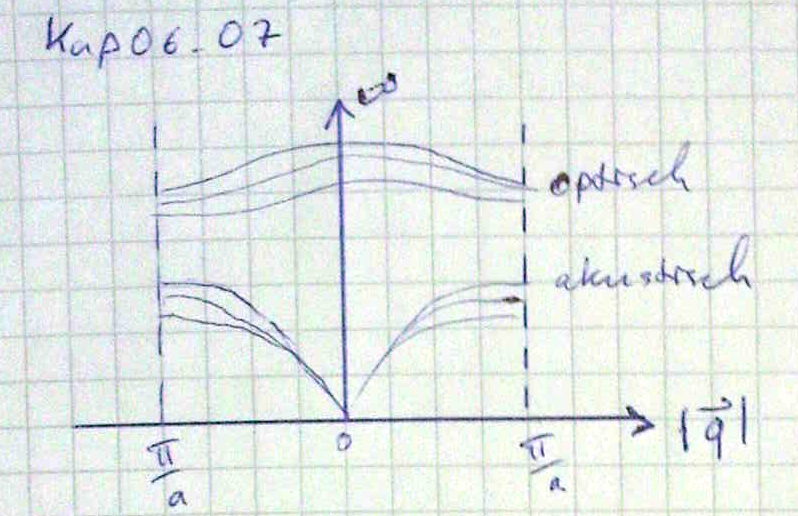
\includegraphics[width=0.75\textwidth]{kap06_07.png}

\section{Quanntisierung elastischer Wellen}

List (EM-Feld) \(\rightarrow\) Photonen \(\rightarrow\) Teilchen
Schall (elastisches Feld) \(\rightarrow\)  Phononen  \(\rightarrow\) Quasiteilchen

Quasiimpuls: \(\hbar \vec q\)
Energie: \(E_{\vec q}=\hbar \omega_{\vec q}\)

Quasiimpuls und seine Energie ist definiert nur in der 1.B.Z.

\[E_{\vec q}=\hbar(n_{\vec q}+\frac{1}{2})\omega_{\vec q}\]

Die Eigenwerte sind quantisiert

\(\frac{1}{2}\hbar \omega_{\vec q}\) ist die Nulpunktenergie des Schwingungszustandes

Energieverluste (inelast. Streuung)

Die Energieverluste könnten wir entweder klassisch (komplexe \(\omega,k\). Damit entspricht der Imaginäre-Teil den Verlusten. 

Oder die Energieverluste werden quantenmechanisch beschrieben (die Zahl der Teilchen ist reduziert). Inelastische Streuung durch Phononen representiert.

Impuls \(\underbrace{\vec k_0}_{\text{Photon}} + \underbrace{\vec B}_{\text{ein Vektor des reziproken Gitters}} = \vec k \pm \underbrace{\vec q}_{\text{Phonon mit Wellenvektor}\vec q}\); Energie \(\hbar \omega_0=\hbar\omega \pm \hbar \omega_q\) 

Ewald Konstruktion
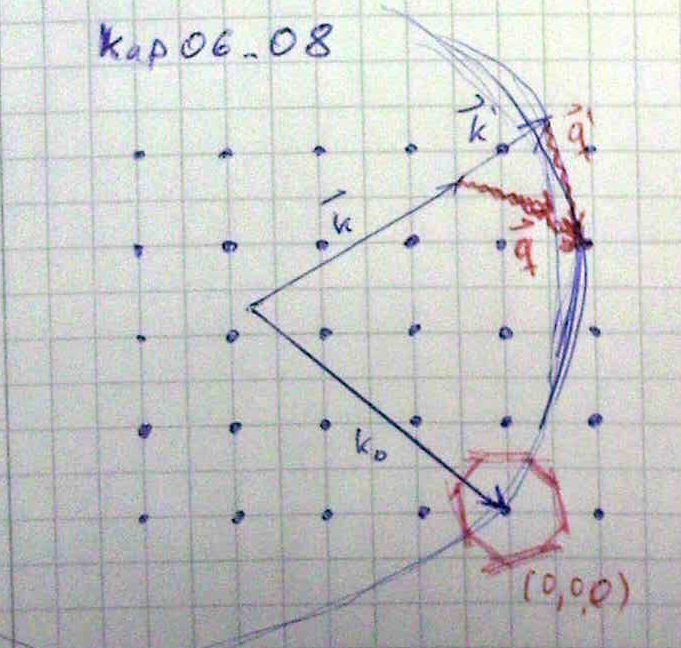
\includegraphics[width=0.75\textwidth]{kap06_08.png}

\(\oplus\) ein Phonon erzeugt
\(\ominus\) ein Phonon absorbiert

\underline{Widerholung} mögliche Streuteilchen (Messsonden)

\begin{itemize}
\item Röntgen-Photonen: \(E\approx 10keV\); ! Phononen: \(E_g\approx 10^{-2}eV\)
\item Elektronen: \(E\approx 100eV\); Nachteil die Eindringtiefe ist gering
\item Neutronen: \(E=\frac{p^2}{2m}=\frac{h^2}{2m\lambda^2} \approx 0,1eV\); können durch den ganzen körper praktisch ungehindert durchfliegen; können mit Phononen interaggieren (innelasische Streuung). 
\end{itemize}

Lichtstreuung: sichtbares List mit \(\lambda_\nu >> a\); \(|\vec k_0|<<|\vec B|\approx \frac{2\pi}{a}\), nur 1.B.Z.

Impulserhaltung: \(\vec k_0=\vec k \pm \vec q\)

Elastische Streuung: Rayleigh-Streuung \(\vec k=\vec k_0\); \(\vec q=0\)

Inelastische Streuprozesse:

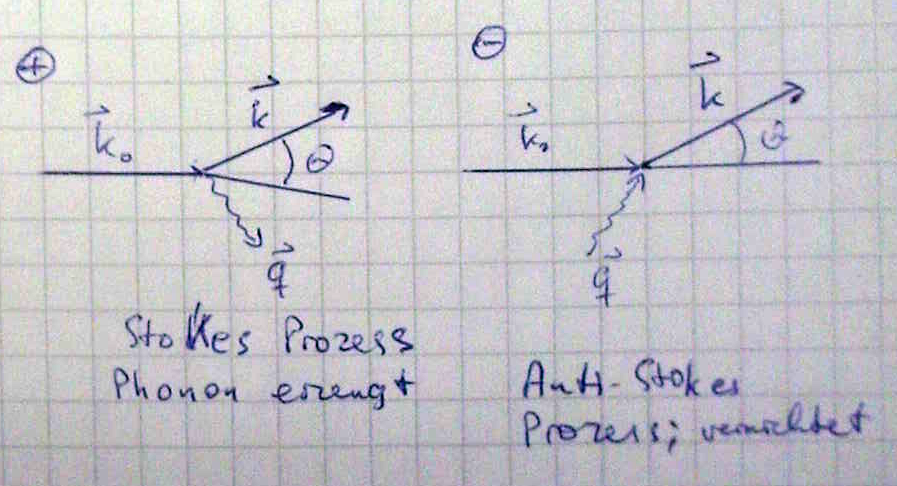
\includegraphics[width=0.75\textwidth]{kap06_09.png}

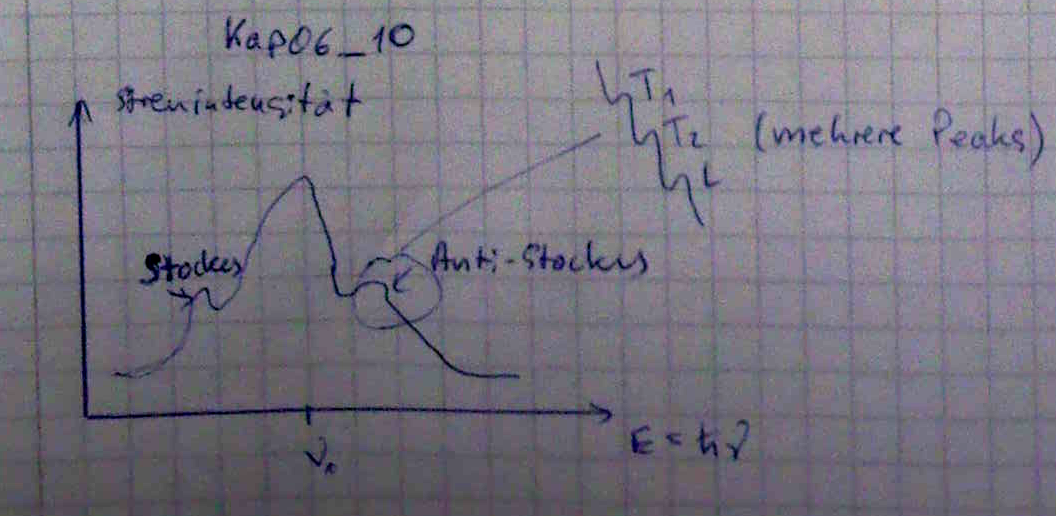
\includegraphics[width=0.75\textwidth]{kap06_10.png}

Streung an akustischen Phononen: Brilloiu-Streuung
Streung an optischen Phononen: Raman Streung

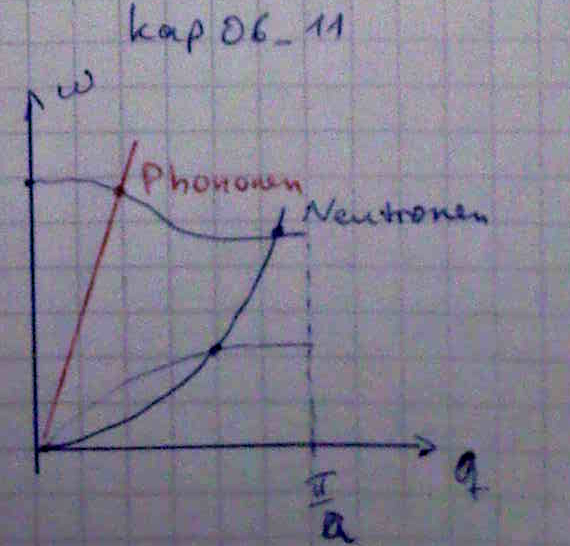
\includegraphics[width=0.75\textwidth]{kap06_11.png}

\section{Zustandsdichte der Phononen}

Theorie eines 3D-Kristalls vorgeschlagen von Born-Karman, 1912 (klassische Theorie)

\(\vec u (x,y,z) = \vec u (x+L_x,y+L_y,z+L_z)\); periodische Randbedingung

Wellen (Moden): \(\vec u = \vec u_0 exp[-i(\omega t-q_xx-q_yy-q_zz)]\)

Periodizität der Atomaren Auslenkung bei \(q_\alpha = m_\alpha\frac{2\pi}{L_\alpha}\); \(\alpha=x,y,z\) und \(m_\alpha\) ganzzahlige Quantenzahl.

\[ e^{iq_\alpha L_\alpha}=1\]

bei einem Kristall mit \(N_\alpha\) Elementarzellen (E.Z.) in \(\alpha\)-Richtung haben wir insgesamt \(N_x,N_y,N_z=N\) E.Z. 3N Lösungen der Bewegungsgleichung; mit p Atome pro E.Z. gibt es 3pN Lösungen der Bewegungsgleichung.

Alle erlaubten wellenvektoren liegen in 1.Brillouin-Zone (1.B.Z.)

'Dichte' \(D(q)\equiv\rho_q\) im reziproken Raum: 

\[\rho_q=\frac{N}{(2\pi)^3/V_z}=\frac{NV_z}{(2\pi)^3}=\frac{V}{(2\pi)^3}\]

\(V_z\)-Das Volumen der E.Z. des realen Gitters.

Zustandsdichte als Funktion der Frequenz \(D(\omega)\): Anzahl von Zuständen pro Einheitsintervall der Frequenz \(\omega\)

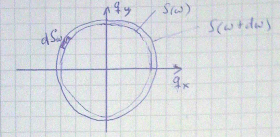
\includegraphics[width=0.75\textwidth]{kap06_12.png}

\[ D(\omega)\cdot d\omega = \rho_q\int^{\omega+d\omega}_\omega d^3q = \rho_q\int^{\omega+d\omega}_\omega dS_\omega\cdot dq_\bot\]

Gruppengeschwindigkeit: \(v_g=\left|\frac{d\omega}{d\vec q}\right| = \left|\underbrace{grad_q\omega}_{\equiv \nabla_q \omega} \right|=\frac{d\omega}{dq_\bot}\)

\[ D(\omega)\cdot d\omega = \frac{V}{(2\pi)^3}\int_{\text{Schalde}\omega=const} \frac{dS_\omega}{v_g}\cdot d\omega\]

Für isotrope Kristalle:

\[ D(\omega)\cdot d\omega = \frac{V}{(2\pi)^3} d\omega \frac{4\pi q^2}{v_g} =\frac{V}{(2\pi)^2} \frac{q^2}{v_g}  d\omega \]

Die Zustandsdichte ist um so größer, je flacher die \(\omega(\vec q)\) verläuft. Kritische Punkte \(\rightarrow\) \underline{van-Hove-Singularitäten} (\(v_g\rightarrow 0\)). Häufigstes vorkommen von Zuständen.

3D \( D(\omega) = \frac{V}{(2\pi)^2} \frac{q^2}{v_g} \); 2D:\( D(\omega) = \frac{A}{(2\pi)^2} \frac{2\pi q^2}{v_g}=\frac{Aq}{2\pi v_g}\) 1D: \( D_1(\omega) = \frac{L}{2\pi}  \frac{2}{v_g}=\frac{L}{\pi v_g} \)

\section{Spezifische Wärme}

\( c=c_{Ges} \frac{N_A}{N}\); \(N_A = 6,022\cdot 10^{23}\); N Elementarzellen E.Z.

\(\left. c\right|_{P=const.}c_p>\left. c\right|_{V=const.}=c_V\); Unterschied zwischen \(c_p\) und \(c_V\) ist in der Realität minimal.

Klassische Theorie: \(c_V = \frac{\partial}{\partial T} U(T)\); \(U\)-innere Energie. Therm. Mittelwert der Energiewerte: \(U\equiv \langle E \rangle = \sum_i p_i\cdot E_i\); \(p_i\)-Wahrscheinlichkeit. Klassisch:

\[ \langle E\rangle = \frac{\int E e^{-\frac{E}{k_B T}}d\Gamma}{\int e^{-\frac{E}{k_B T}}d\Gamma}\]

\(d\Gamma=dx\cdot dy\cdot dz\)-Phasenraum

harmonischer Oszillator: \(\langle E_{Oszi} \rangle = k_B T\)
3pN Gitterschwingungen: \(c_V = 3pNk_B\) Dulong-Petit-Gesetz (1819)

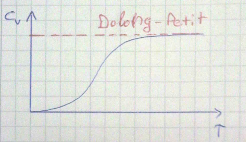
\includegraphics[width=0.75\textwidth]{kap06_13.png}

\(c_V=3R=3\cdot 8,3\frac{J}{mol\cdot K} = 24,9\frac{J}{mol\cdot K} = const.\); \(R\)-univers.Gaskonstante

Quantentheorie: Erste Erklärungsversuch von Einstein (1906) und zweiter und besserer Versuch von Debye (1912). 

Zustand n mit \(E_n=(n+\frac{1}{2})\hbar \omega\); Boltzmann-Verteilung:

\[ p_k=\frac{e^{-\frac{E_n}{k_B T}}}{\sum^\infty_{n=0} e^{-\frac{E_n}{k_B T}}} = e^{-\frac{n \hbar \omega}{k_BT}}\left[1- e^{-\frac{\hbar \omega}{k_BT}}\right]\]


Nenner \(=e^{-\frac{\hbar \omega}{2k_BT}}\sum^\infty_{n=0} \left[e^{-\frac{\hbar \omega}{2k_BT}}\right]^n= e^{-\frac{\hbar \omega}{2k_BT}}\sum^\infty_{n=0} \left[1- e^{-\frac{\hbar \omega}{k_BT}}\right]^{-1}\);mit  \(\sum^\infty_0 x^n = \frac{1-x^{n+1}}{1-x}\approx \frac{1}{1-x}\); \(n\rightarrow \infty,x\rightarrow 0\)


\[ U \equiv \langle E_n \rangle = \sum^\infty_{n=0} p_n\cdot E_n = \left[1- e^{-\frac{\hbar \omega}{k_BT}}\right]\hbar \omega \sum^\infty_{n=0}(n+\frac{1}{2})\left[\underbrace{1- e^{-\frac{\hbar \omega}{k_BT}}}_{x}\right]^n\]

\(\sum_n x^nn=x\frac{d}{dx}\sum_n x^n = \frac{x}{(1-x)^2}\)

\[ \langle E_n \rangle = \hbar \omega \left[ \frac{1}{e^{-\frac{\hbar \omega}{k_BT}}-1}+\frac{1}{2}\right]\]

mit \(E_n=\hbar\omega(n+\frac{1}{2})\)

\(\langle n \rangle \frac{1}{e^{-\frac{\hbar \omega}{k_BT}}-1}\); Bose-Einstein Faktor; \(E(\omega,T) = \hbar \omega[\langle n \rangle + \frac{1}{2}]\)


\section{Debye-Näherung}

Debye-Näherung kannman für isotrope Festkörper anwenden mit \(p=1\Rightarrow \omega = v_g\); \(v=v_g\). Betrachte nur akustische Phononen.

\[  D(\omega)\cdot d\omega = \frac{V}{(2\pi)^2} \frac{\omega^2}{v^3}  d\omega \]

Zustandsdichte pro Phononenzweig (Ast)

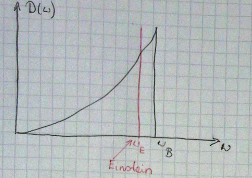
\includegraphics[width=0.75\textwidth]{kap06_14.png}

\(N=\int^{\omega_D}_0\frac{V}{(2\pi)^2} \frac{\omega^2}{v^3}  d\omega = \frac{V\omega^3_D}{6\pi^2 v^3}\); \(\omega_D=\frac{v}{a}\quad ^3\sqrt{6\pi^2}\); \(\frac{V}{N}\approx a^3\)-Gitterkonstante

\(\omega \propto vg\)

Abscheidefrequenz \(\omega_D \Rightarrow\) Debye-Frequenz.
\[\boxed{\omega_D=\frac{v}{a}\quad ^3\sqrt{6\pi^2}}\]

\(D(\omega)= \frac{v\omega^2}{2\pi^2}\left(\frac{1}{v_L^3}+\frac{2}{v^3_T} \right)=\frac{3}{2\pi^2}\frac{\omega^2v}{v_D^3} \); \(\frac{3}{v_D^3}\equiv\frac{1}{v_L^3}+\frac{2}{v_T^3}\); typisch \(v_L\approx \frac{3}{2}v_T\)

Schwingungsenergie des Kristalls: \(v(T) = \int_0^\infty D(\omega) E(\omega,T) d\omega\)

Spezifische Wärme: \(c_V = \frac{\partial v(T)}{\partial T}\); 

\[v=\frac{v}{2\pi^2}\underbrace{\frac{1}{v^3}}_{\frac{3N}{v}\frac{6\pi^2}{\omega_D^3}}\int_0^\infty \omega^2 E(\omega,T) d\omega=\frac{9N}{\omega_D^3}\int_0^\infty\frac{\hbar \omega^3 d\omega}{e^{\frac{\hbar \omega}{k_B T}}-1}\]

Debye-Temperatur: \(\theta_D = \frac{\hbar \omega_D}{k_B}\) mit \(y= \frac{\hbar \omega}{k_BT}\), Debye-Formel:

\[ c_V = 9Nk_B\left(\frac{T}{\theta_D}\right)^3 \int_0^{\theta_D/T}\frac{y^4e^ydy}{(e^y-1)^2}\]


Debye-Temperaturen:

\begin{tabular}{c|ccccccc}
 &\(C_{\text{Diamant}}\)&Be&Si&Al&Cu&Ar&He\\
\(\theta_D,K\)&2230&1000&640&430&340&92&25
\end{tabular}

a) \(T<<\theta_D\) tiefen Temperaturen \(\rightarrow\) Einstein-Theorie
b) \(T>>\theta_D\) hohen Temperatruren  \(\rightarrow\) klassische Thermodynamik

a): \(y\rightarrow \infty\), \(\int_0^\infty \frac{y^4e^ydy}{(e^y-1)^2} = \frac{4\pi^4}{15}\); \(c_v = \frac{12\pi^4}{5}Nk_B\left(\frac{T}{\theta_D}\right)^3 \approx T^3\); \(T^3\)-Gesetz

b): \(y\rightarrow 0\) , \(\int_0^{\theta_D/T}...dy \approx = \int_0^{\theta_D/T}\frac{y^4\cdot 1}{(1+y-1)}dy= \int_0^{\theta_D/T}y^2dy=\frac{1}{3}\left(\frac{T}{\theta_D}\right)^3\), \(c_V=3Nk_B\), Dulong-Petit Gesetz.

\section{Anharmonische Effekte}

Klassisch gesehen ein Anharmonischer Effekt ist eine Abweichung von harmonischen Potential. 

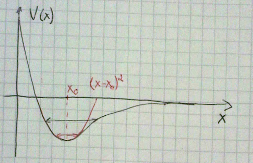
\includegraphics[width=0.75\textwidth]{kap06_15.png}

Auslenkungen sind nicht mehr klein! dann bekommt man die anharmonische Effekte. 

Quantenmechanisch die Anharmonischen Effekte kann man als Wechselwirkung zwischen Phononen beschreiben (Phononenstoßprozesse)

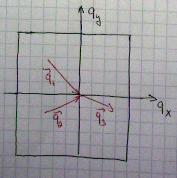
\includegraphics[width=0.75\textwidth]{kap06_16.png}

Normale Prozesse: \(\vec q_1+\vec q_2=\vec q_3\)

Umklapp-Prozesse: \(\vec q_1+\vec q_2=\vec q_3+\vec B\)

\subsection{Therminsche Ausdehnung}
klassisch: \(U(x)\approx cx^2-\overbrace{gx^3-fx^4}^{\text{anharmonische Terme}}+...\);Auslenkung: \(\langle x\rangle = \frac{\int_0^\infty dx x e^{\frac{-U(x)}{k_BT}}}{\int_0^\infty dx e^{\frac{-U(x)}{k_BT}}}\) aus der Thermodynamik ergibt sich:

\[\rightarrow \langle x \rangle \approx \frac{3g}{4c^2}k_B T\]

Wärmeausdehnungskoeffizient:  \(\alpha\equiv \frac{1}{l} \left( \frac{\partial l}{\partial T}\right)_p=\frac{1}{3} \frac{1}{v}\left( \frac{\partial v}{\partial T}\right)_p\); \(l\propto \langle x \rangle\);
  \(\left( \frac{\partial V}{\partial T}\right)_p=-\left( \frac{\partial V}{\partial p}\right)_T\cdot \left( \frac{\partial p}{\partial T}\right)_v\); \(\frac{1}{B}=-\frac{1}{V}\left( \frac{\partial V}{\partial p}\right)_T\)


\(\left( \frac{\partial V}{\partial T}\right)_p = \frac{V}{B}\left( \frac{\partial p}{\partial T}\right)_V\); 

\[\boxed{\alpha = \frac{1}{3B}\left( \frac{\partial p}{\partial T}\right)_V }\]


\( p = - \left( \frac{\partial F}{\partial T}\right)_T\); \(F\)-freie Energie;

 \[ p = -\frac{\partial}{\partial V}(E_0+E_z) -\sum_q\frac{\partial(\hbar \omega_g)}{\partial V}\langle n_g(T)\rangle\] 


\(E_0\)-Energie des Grundzustands; \(E_z\)-Nullpunkt-Schwingungn \(\langle n_g(T)\rangle\)-Mittlere Zahl von Phononen

für harmonischen Kristall: \(c_P=c_V\)

 
\[\alpha = \frac{1}{3B}\sum_q\left[-\frac{V}{\omega_g}\frac{\partial \omega_g}{\partial V}  \right]\underbrace{\frac{1}{V}\hbar \omega_g\frac{\partial}{\partial T}\langle n_g(T)\rangle}_{c_v(q)}\]
\[ = \frac{\partial(ln\omega_g)}{\partial V} \equiv \gamma_q\]

\(\gamma_q\)-Grüneisenzahl
Grüneisenparameter \(\gamma_q\equiv \frac{1}{c_V}\sum_q\gamma_qc_V(q)\approx const. \approx 1\div 3\)

\[\boxed{\alpha = \frac{\gamma c_V}{3B}\approx 10^{-5}K^{-1}}\]

\(\alpha\approx T^3\) für \(T<<\theta_D\); \(\alpha\approx const\) für \(T>>\theta_D\)

\subsection{Wärmeleitfähigkeit}

\[ \kappa = \kappa^{ph}+\kappa^{el}\]

Wärmestromdichte \(\vec J_T = -\kappa\nabla T\), nach den kinetischer Gastheorie \(\kappa = \frac{1}{3}vlc_v = \frac{1}{3}v^2\tau c_v\); \(l\)-Länge; \(\tau\)-mittlere Zeit zur Phononenstöße

\section{Klassisches Drude Modell}

\begin{enumerate}
\item \(e^{-}\) haben keine WW mit dem Gitterpotential
\item \(e^{-}e^{-}\) Wechselwirkung
\item äußere Felder wirken auf die \(e^{-}\)
\item  \(e^{-}\) \(\frac{1}{2}m\langle v^2\rangle =\frac{3}{2}kT\)
\item \(\tau\) Stoßanzahl, Rekombintionszeit \(\frac{1}{\tau}\) \(\frac{dt}{\tau}=\) Wahrscheinlichkeit für Stöße
\end{enumerate}

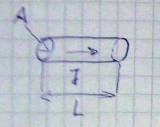
\includegraphics[width=0.75\textwidth]{kap06_17.png}

\(\vec J=\rho j\); \(j=\sigma\vec E\); \(j=\frac{I}{A}\); \(E=\frac{V}{L}\); \(\Rightarrow V=RJ\); \( \frac{\rho L}{A}\)

\[ j = -ne\vec v_D\]

\[\left. \vec v\right|_{t=t_1}=v'_{t=t_0}-\frac{e\vec E t}{m} \]

\begin{align}
\vec v_D &= \langle \vec v \rangle  = \langle v_0\rangle -\frac{eE\tau}{m} \\
&=\frac{eE\tau}{m}
\end{align}


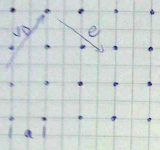
\includegraphics[width=0.75\textwidth]{kap06_18.png}

\(\vec j = \frac{ne^2\tau}{m}\vec E\); \(\sigma = \frac{ne^2\tau}{m}\); \(\tau = \frac{m}{\rho n e^2}\)


\(a\approx 10^{-10}m\); \(\tau = \frac{a}{\sqrt{\langle v\rangle }}\approx \frac{a}{\sqrt{\frac{3k_BT}{m}}}\)
\(\Rightarrow \tau = 10^{-14}s\)

\(\left. a\right|_{300K} = n 10^{23}\); \(\sigma = 10^{5}\frac{1}{\Omega cm}\)

\(\sqrt{\frac{3k_BT}{m}}\approx 10^5\frac{m}{s}\) ; \(l=\frac{\langle v^2\rangle }{\tau}\approx 1 bis 10\cdot 10^{-10}m\)

\(\left. l \right|_{4K}\approx 100\mu m\)

\subsection{Impuls Reelaxation}

\(\vec v = \frac{\vec p}{m} \Rightarrow \vec j = -\frac{ne\vec p}{m}\) Stoßwahrscheinlichkeit: \(\frac{dt}{\tau}\)
keine Stoßwahrscheinlichkeit \(1-\frac{dt}{\tau}\)


\begin{align}
p(t+dt) &= (1-\frac{dt}{\tau})[p(t) + F(t)dt+\mathcal O(dt^2)]\\
&\approx p(t) -\frac{dt}{\tau}p(t) + F(t)dt+\mathcal O(dt^2)
\end{align}

\[\boxed{\frac{dp(t)}{dt}=-\frac{p(t)}{\tau}+F(t)}\]


\underline{Hall-Effekt}
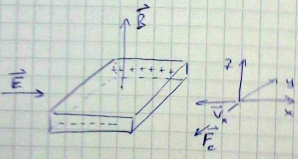
\includegraphics[width=0.75\textwidth]{kap06_19.png}

\[ F = -eE-e\vec v\times \vec B\]

\[E_\gamma = v_xB_z = -\frac{1}{en}j_x B_z = R_H j_xB\]

\[\boxed{R_H=-\frac{1}{en}}\]

Kupfer \(Cq\) - \(R_H=-5,3\cdot 10^{-11}\frac{m^3}{c}\)
Aluminium \(Al\) - \(R_H=+9,9\cdot 10^{-11}\frac{m^3}{c}\)



\begin{align}
\frac{dp}{dt} &= -eE - \frac{e}{m}\vec p \times \vec B - \frac{\vec p}{\tau} = 0\\
0&=-eE_x - \frac{e}{m}p_yB - \frac{p_x}{\tau}\\
0&=-eE_y - \frac{e}{m}p_xB - \frac{p_y}{\tau}
\end{align}

\[ \Rightarrow \sigma E_x = \omega_c \tau j_y + j_x\]
\[ \Rightarrow \sigma E_y = -\omega_c \tau j_y + j_y\]

Zyklotronfrequenz
\[ \omega_c = \frac{e}{m}B \]

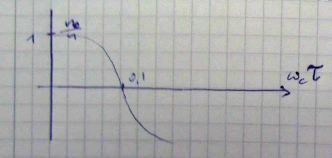
\includegraphics[width=0.75\textwidth]{kap06_20.png}

Laut Drude sollte \(\omega_C\tau \propto B\) sein, ist es aber nicht (warum, nicht kapito)

\subsection{Wechselstromleitfähigkeit}

\(\frac{dp}{dt} = -\frac{\vec p}{\tau} - e\vec E\); \(E(t) = Re\{E(\omega)e^{-i\omega t}\}\)

Versuch der Lösung

\[ p(t) = - Re\{p(\omega)e^{-i\omega t}\} \]
\( -i\omega \vec p(\omega) = -\frac{\vec p(\omega)}{\tau}-e\vec E\); \(\vec j = -\frac{ne}{m}\vec p\)
\(\Rightarrow j(t) =  Re\{j(\omega)e^{-i\omega t}\}\)

\[ j(\omega) = -\frac{ne}{m} p(\omega) = \frac{ne^2}{m}\frac{\vec E(\omega)}{\frac{1}{\tau}-i\omega}\equiv\sigma(\omega)\vec E(\omega) \]

\[\boxed{\sigma(\omega) = \frac{\sigma_0}{1-i\omega\tau}}\]

Magnetfeld \(H(\omega) \approx 0\); \(\frac{v}{c}<< 1\); \(v_D\approx 10^{-3}\frac{m}{s}\)

Maxwell-Gleichungen \(\lambda = \frac{2\pi c}{\omega}>> e \)
Ampersche Gesetz: \(\vec \nabla \times \vec H = j + \epsilon_0\frac{\partial E}{\partial t}\)

\begin{align}
\vec \nabla \times \vec \nabla \times \vec E = -\nabla^2 E &= i\omega \mu_0\sigma \vec E - i\omega \epsilon_0\vec E\\
&=w^2 \epsilon_0\mu_0\epsilon(\omega) \vec E
\end{align}

\[\epsilon (\omega) = 1+ \frac{i\sigma(\omega)}{\epsilon_0 \omega}\]


\begin{enumerate}
\item hohee Frequenzen \(\sigma(\omega) = \omega_0\frac{1+i\omega\tau}{1+\omega^2\tau^2}\approx\sigma_0\frac{i}{\omega\tau}\); \(\Rightarrow \epsilon(\omega) = 1-\frac{\sigma_0}{\epsilon_0\tau\omega^2}=\frac{\omega^2_0}{\omega^2}\)

Die Plasmafrequenz, ist gerade die Frequenz wo die \(e^-\)  dem Feld noch folgen können. 
\[ \omega_p = \frac{ne^2\tau}{m\epsilon_0 \tau}=\frac{ne^2}{m\epsilon_0}\]
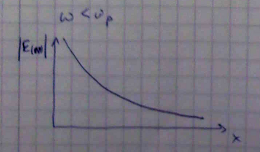
\includegraphics[width=0.75\textwidth]{kap06_21.png}

\item kleine Frequenzen \(\omega\tau << 1\)

\[\sigma (\omega) = \sigma_0 \frac{1+i\omega\tau}{1+\omega^2\tau} =  \sigma_0(1+i\omega\tau)\]

\[ \epsilon(\omega) = 1+\sigma(mega)\frac{1}{\epsilon_0\omega} = 1 + \sigma_0(\underbrace{\frac{i}{\epsilon_0\omega}}_{\epsilon_2}-\underbrace{\frac{\tau}{\epsilon_0}}_{\epsilon_1})\]

\[ \epsilon(\omega) = = i\epsilon_2\]

\[ k = \frac{\omega}{c}\sqrt{\epsilon(\omega)} =  \frac{\omega}{c}\sqrt{\frac{\sigma_0}{\epsilon_0 \omega}}\frac{1+i}{\sqrt 2} = \frac{1}{s}(1+i)\]

\[s = c\sqrt{\frac{2\epsilon_0}{\sigma_0\omega}}\]

\(s\) ist der Skin oder Leitschichtdicke (Dimension Länge) oder der Skin-Effekt. Der Strom fließt nun noch an der Oberfläche des Leiters. 

\end{enumerate}


1853 Widermann-Franz. Die Wärmeleitfähigkeit und die Leitfähigkeit ist zur Temperatur proportional:

\[ \frac{\kappa}{\sigma} = LT\]

\(L\)-Loreznzahl zwischen \(2,2-2,8\cdot 10^{-3}\frac{\omega\Omega}{K^2}\)

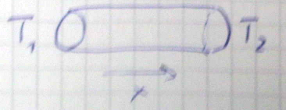
\includegraphics[width=0.75\textwidth]{kap06_22.png}

\(j^T = \kappa \nabla T\)

\begin{align}
j^T_x &= \langle \frac{1}{2}v_x [u_x(x-v\tau)i-u_c(x+v\tau]\rangle \\
&= n\langle v_x^2\rangle \tau \frac{du_e}{dT}(-\frac{dT}{dx}
\end{align}

\(c_v = n\frac{du}{dT}\); \(\rangle v^2\rangle  = \langle v_x^2\rangle = \langle v^2_x\rangle =\langle v_z^2\rangle \)

\[ j^T = \underbrace{\frac{1}{3}v^2\tau c_v}_{\kappa = \frac{1}{3}v^2\tau c_v=\frac{1}{3}lvc_v} \]

\[ LT =  \frac{\kappa}{\sigma} = \frac{c_v}{ne^2} \frac{mv^2}{3} \]
\(\Rightarrow c_v = \frac{3}{2} nk_B\)

\[ L =\frac{\kappa}{\sigma}\frac{3}{2} nk_B \frac{k^2_B}{K^2} T = 1,1\cdot 10^{-3}\frac{\omega\Omega}{K^2}\frac{mv^2}{2} = \frac{3}{2}k_B T\]

tatsächlich: \(c^2_v\) Fatkro 100 kleiner, \(v^2\) ist ein Faktor 100 größer



\section{Sommerfeld-Theorie der Metalle}

Klassische, Ideales Gas Maxwell-Bolzmann Veirteilung

\[ f_{MG} = (v) = n\left(\frac{m}{2\pi kT}\right)^{3/2}e^{-\frac{mv^2}{k_B T}} \]

Pauliprinzip:

Fermi Dirac Verteilung

\[ f_{FD} = f(v) = \left(\frac{m}{2\pi \hbar}\right)^3 \frac{2}{e^{\frac{mv^2/2-\mu}{k_BT}}+1} \]

\(n=\int_V f(v) dV\); \(k_BT_0 = \nu\)

Zustandsdichte des freien Elektronen Gases:

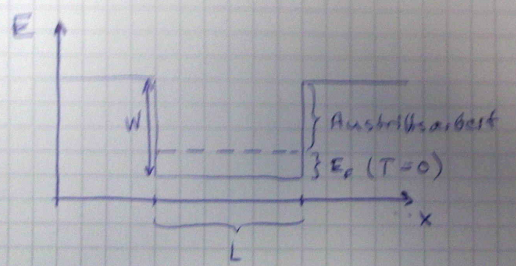
\includegraphics[width=0.75\textwidth]{kap06_23.png}

N Elektronen
SchrGl: \(-\frac{\hbar}{2m} \nabla \psi(\vec r) = E \psi(\vec r)\); \(\psi(\vec r) = \frac{1}{\sqrt{V}} e^{-\vec k\vec r}\); \(1=\int_V|\psi(\vec r)|^2dV\); \(E=\frac{\hbar^2k^2}{2m}\);

Peridizitätsbedingung:  \(\psi(x,y,z) = \psi(x+L,y,z)\)

\(k_i=\frac{2\pi}{L}m_i\) \(i=x,y,z\); \(m=1,2,3\)

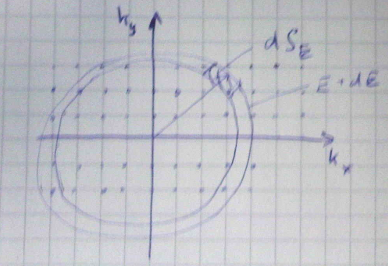
\includegraphics[width=0.75\textwidth]{kap06_24.png}

\[\mathcal D(E) dE = \frac{V}{(2\pi)^3}\int^{E+dE}_E d^3 k = \frac{V}{(2\pi)^3} \frac{1}{\hbar} \int_{E=const.} \frac{dS_E}{v_g}\]

\(\rho_x = \frac{V}{(2\pi)^3}\)

Gruppengeschwindigkeit: \(v_g = \frac{\partial E}{\partial(\hbar k} = \frac{\hbar k}{m}\)

Randbemerkung: \(\frac{1}{v_g}\int dS_E = \frac{1}{v_g}-4\pi k^2\)

\[\mathcal D_\uparrow(E) = \frac{V}{(2\pi)^3}\frac{1}{\hbar} \frac{m}{\hbar k}4\pi k^2 = \frac{(2m)^{3/2}}{4\pi^2\hbar^2} V\sqrt{E}\]

Volumen normierte und mit 2 \(e^-\) besetzte Zustandsdichte:

\[ \mathcal D(E) = \frac{1}{V} (\mathcal D_\uparrow + \mathcal D_\downarrow) = \frac{(2m)^{3/2}}{2\pi^2\hbar^2}\sqrt{E}\]

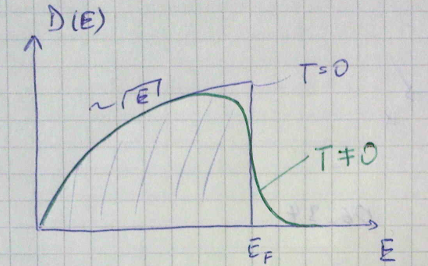
\includegraphics[width=0.75\textwidth]{kap06_25.png}

\(\rho^\propto_k=\left(\frac{L}{2\pi}\right)^\propto\)

\(D^{2D}=\frac{m}{\pi \hbar^2}\); \(D^{1D}(E) = \frac{1}{\pi\hbar} \sqrt{\frac{2}{E}}\)

\[f(E,T=0) = \begin{cases}
  1: & E<\mu \\
  \frac{1}{2}: & E=\mu \\
  0: & E>\mu 
\end{cases}
\]

\(\mu = \left(\frac{\partial F}{\partial N}\right)_{T,V}=E_F(T=0)\)

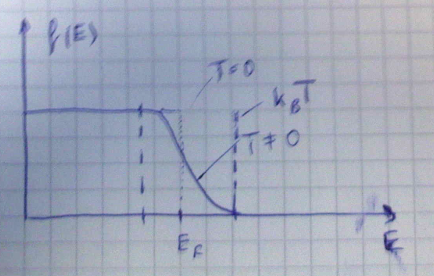
\includegraphics[width=0.75\textwidth]{kap06_26.png}

\[n=\frac{N}{V}=\int_0^\infty \mathcal D(E) f(E,0)dE = \int_0^{E_F}\]

\[E_F = \frac{\hbar^2}{2m}(3\pi^2n)^{2/3}\]

Fermi-Energie: \(E_F = \frac{\hbar^2}{2m}(3\pi^2 n)^{2/3}\) mit Elektronendichte \(n=\frac{N}{V}\)
Fermi-Wellenvektor \(k_F=(3\pi^2n)^{1/3}\)
Fermi Impuls: \(p_F = \hbar k_F\)
Fermi-Geschwindigkeit \(v_F = \frac{\hbar}{m}(3\pi^2 n)^{1/3}\)
Fermi Temperatur \(T_F = \frac{E_F}{k_B}\)


\begin{tabular}{cccccc}
&\(n/10^{6}m^{-3}\)&\(k_f/A^{-1}\)&\(v_F10^{6}\frac{m}{s}\)&\(E_F/eV\)&\(FT/K_F\)\\
Al&18,1&1,8&2,0&11,7&135000\\
Cu&8,5&1,4&1,6&7,0&82000\\
Ag&5,9&1,2&1,4&5,5&64000
\end{tabular}


\[\boxed{\mu(T)\approx E_F [1-\frac{\pi^2}{12}\left(\frac{T}{T_F}\right)^2]}\]


TODO Einleitende Abbildungen möglich am anfang von Sommerfeldtheorie einfügen


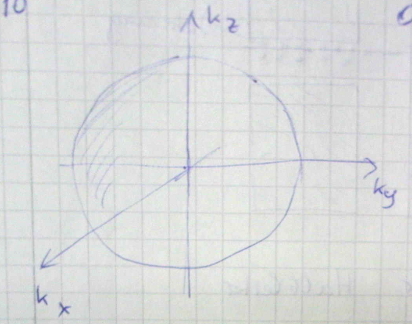
\includegraphics[width=0.75\textwidth]{kap06_27.png}


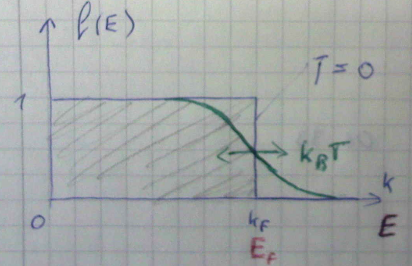
\includegraphics[width=0.75\textwidth]{kap06_28.png}
Kurze Einleitung was die Quantennatur der Theorie ist (Pauliprinzip, Besetzung in der Fermikugel, nur an der Fermikante befindliche elektronen sind relevant für verschiedene Effekte)

\subsection{Spezifische Wärme}

\(c_V = \frac{\partial }{\partial T}U(T)\) mit \(U\) als innere Energie

\begin{align}
c_V &= \frac{\partial }{\partial T}U(T)\\
&= \frac{\partial }{\partial T}\int_0^\infty ED(E)f(E,T)dE\\
&=\frac{\partial }{\partial T}\frac{1}{2\pi^2}\left(\frac{2m}{\hbar}\right)^{3/2}\int_0^\infty\frac{E^{3/2}dE}{e^{\frac{E-\mu}{k_BT}}-1}
\end{align}

\begin{align}
D(E)&=\frac{(2m)^{3/2}\sqrt{E}}{2\pi^2\hbar^3}\\
&=\frac{3}{2}n\sqrt{E}\left[\frac{\hbar^2}{2m}(3\pi^2 n)^{2/3}\right]^{-3/2}\\
&= \frac{3}{2}\frac{n}{E_F}\left(\frac{E}{E_F}\right)^{1/2}
\end{align}


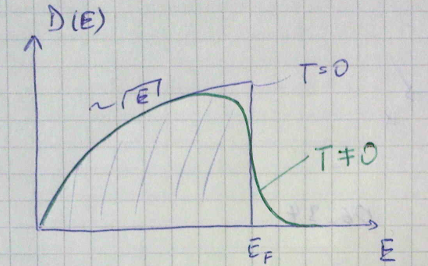
\includegraphics[width=0.75\textwidth]{kap06_25.png}

'grobe'-Rechnung:

\begin{align}
U(0) &= \int_0^{E_F}ED(E)dE\\
&= \frac{3}{2}\frac{n}{E_F^{3/2}}\frac{2}{5}E^{5/2}\\
&=\frac{3n}{5}E_F\\
&=\frac{3n}{5}k_BT
\end{align}

Temperaturabhängige Anteil der innerer Inergie:

\[\delta U(T) = U(T)-U(0) \approx nk_BT\frac{T}{T_F} = nk_B \frac{T^2}{T_F}\]

\(\frac{T^2}{T_F}\) der Bruchteil der Elektronen der die thermische Energie \(k_BT\) pro Elektron aufnehmen kann

\(c_V \approx \frac{\partial}{\partial T}[\delta U(T)] = \frac{2nk_BT}{T_F}\) ist um Faktor \(\frac{T}{T_F}\) kleiner als mit einem klass. Gas.

exaktere Näherungslösung:  \(U(T) \approx U(0) +\frac{\pi^2}{6}D(E_F)(k_BT)^2\); \(c_V=\gamma T\); mit Sommerfeldkonstanten \(\gamma = \frac{\pi^23nk_B}{3T_F2}\)

Die gesamte spezifische Wärme:

\[c_V^{\text{ges}} = c_V^{el}+c_V^{ph} = \gamma T + \begin{cases}
 \beta T^3,  & T<<\theta_D\\
 3R=const,  & T>\theta_D
\end{cases}\]


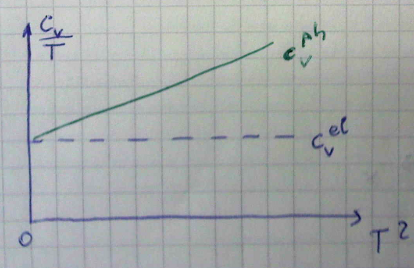
\includegraphics[width=0.75\textwidth]{kap06_30.png}

Offene Fragen nach Sommerfeld-Modell:

\begin{enumerate}
\item Warum collidieren \(e^-\)-nen nicht mit Ionen?
\item Warum teilen/unterscheiden wir zwischen Metalle, Halbleiter, Isolatoren?
\item Warum wechselwirken  \(e^-\)-nen nicht mit einander?
\end{enumerate}

Die ersten zwei Fragen sind von Bloch-Theorie beantwortet. Die dritte Frage - Fermi-Flüssigkeiten (komplizierte QM-Theorie)


\section{Energiebänder}

Oder warum unterscheiden wir zwischen Halbleiter, Leiter und Isolatoren.

'gute' Leiter: \(\rho\approx 10^{-10}\Omega \cdot cm\)
'gute' Isolator:  \(\rho\approx 10^{22}\Omega \cdot cm\)

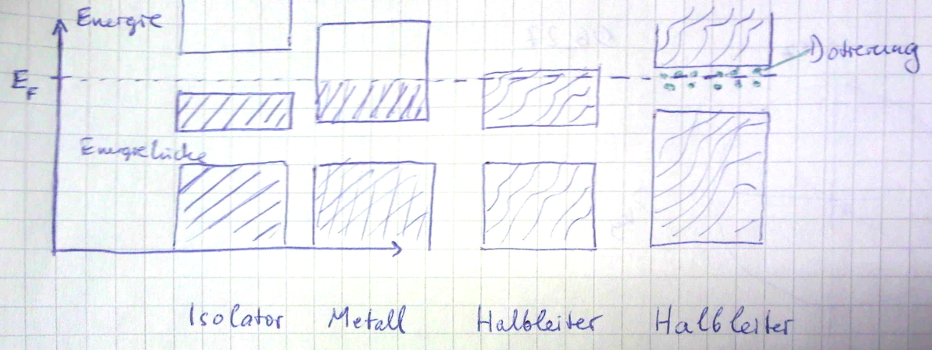
\includegraphics[width=0.75\textwidth]{kap06_31.png}

\underline{1 Beispiel}: Model des nahezu freien Elektronen

\(E_x=\frac{\hbar^2k^2}{2m}\); Wellenfunktion \(\psi_{\vec k} = e^{i\vec k\vec r}\)

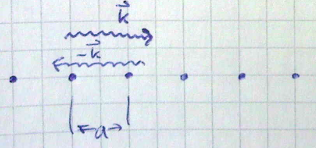
\includegraphics[width=0.75\textwidth]{kap06_32.png}

Laue (Bragg-Reflekton) \(-\vec k+\vec G = \vec k\) mit reziproken Gitter \(\vec G\)

\[ (-\vec k +\vec G)^2 = \vec k^2 \Rightarrow 2kG = G^2; \qquad k=\frac{G}{2}=\pm \frac{\pi}{2}n_G\]

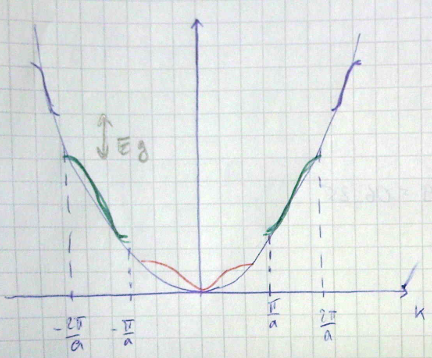
\includegraphics[width=0.75\textwidth]{kap06_33.png}

Zwei verschiedene Stehende Wellen:

\[ \psi_+ \propto e^{i\frac{\pi x}{a}}+e^{-i\frac{\pi x}{a}}=2cos\frac{\pi x}{a} \]
\[ \psi_- \propto e^{i\frac{\pi x}{a}}-e^{-i\frac{\pi x}{a}}=2isin\frac{\pi x}{a} \]

Gruppengeschwindigkeit \(v_G = \frac{\partial E_k}{\partial p} = \left.\frac{\hbar k}{m}\right|_{k=\pm\frac{\pi}{a}}=^!0;\)

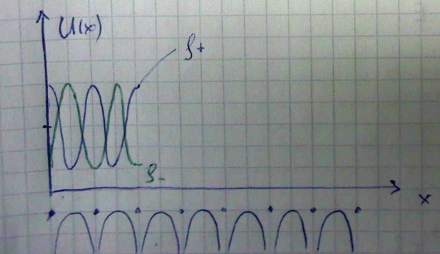
\includegraphics[width=0.75\textwidth]{kap06_34.png}

\[\rho_+=|\psi_+|^2 \propto cos^2\frac{\pi x}{a} = \frac{1}{2}(1+cos^2\frac{2\pi x}{a})\]
\[\rho_-=|\psi_-|^2 \propto sin^2\frac{\pi x}{a} = \frac{1}{2}(1-cos^2\frac{2\pi x}{a})\]


Wahrscheinlichkeitsdichte \(\psi^*\psi=|\psi|^2\); \(\rho_0=1e=e^{-ikx}e^{ikx}e\)

Erwartungswert der Potentiellen Energie: \(E_{\rho_+}<E_{\text{frei}}<E_{\rho_-}\), \(U(x)=U cos\frac{2\pi x}{4}\); 

\begin{align}
E_g &= \frac{1}{a}\int dx U(x)[|\psi_-|^2-|\psi_+|^2]\\
&=\frac{2U}{a}\int_0^a dx cos\frac{2\pi x}{4}\frac{1}{2}[1-cos\frac{2\pi x}{a}-1-cos\frac{2\pi x}{a}]\\
&= \frac{2U}{a}\int_0^a dx cos^2\frac{2\pi x}{a}\\
&= \frac{U}{a}\int_0^a dx (1+cos\frac{4\pi x}{a})\\
&=\frac{U}{a}\left.(x+\frac{a}{4\pi}sin\frac{4\pi x}{a})\right|_0^a \\
&\equiv U = E_B-E_A
\end{align}


Elektronen in einem periodischen Potential (QM)
\[ H\psi(\vec r) = [-\frac{\hbar^2}{2m}\nabla+\tilde V(\vec r) ]\psi (\vec r) = E\psi(\vec r) \]

Translationsinvariant: \(\tilde V(\vec r) = \tilde V(\vec r+\vec l)\)

Entwicklung nach reziproken Gittervektoren \(\vec G\) (blochscher Ansatz)

\[\tilde V(\vec r) = \sum_G\tilde V_G\cdot e^{i\vec G\vec r}\]
\[\psi(\vec r) = \sum_{k}c_ke^{ikr}\]
Einsetzen in die SGL:

\[\sum_{\vec k}\frac{\hbar^2 k^2}{2m}c_ke^{i\vec k\vec r}+\sum_{k',\vec G}c_{k'}\tilde V_G e^{i(k'+G)\vec r}\equiv \sum_kc_ke^{i\vec k\vec r}\]
Umbenennung (summe über alle \(k'\)): \(k'+\vec G = k \rightarrow \)

\[0=\sum_{\vec k}e^{i\vec k\vec r}\underbrace{\left[(\frac{\hbar^2 k^2}{2m}-E)c_k+\sum_G\tilde V_G c_{\vec k-\vec G}\right]}_{=0}\]


\[(\frac{\hbar^2 k^2}{2m}-E)c_k+\sum_G\tilde V_G c_{\vec k-\vec G}=0\]

Dieser Satz algebraischer Gleichungen ist die Darstellung der Schrödigner Gleichung im \(\vec k\)-Raum \(\Rightarrow\) \(E_k\)-Energie Eigenwert.

\begin{align}
\psi_k(\vec r) &= \sum_{\vec G}c_{\vec k-\vec G}e^{i(\vec k-\vec G)\vec r}\\
&= \underbrace{e^{i\vec k\vec r}}_{\text{ebene Welle}}\underbrace{\sum_{\vec G}c_{\vec k-\vec G}e^{-i\vec G\vec r}}_{U_k(\vec r)}\\
&= U_k(\vec r)e^{i\vec k\vec r}
\end{align}

Bloch Theorem: Die Eigenfunktionen der SG. für ein periodisches Potential sind das Produkt aus einer ebenen Welle und einer Funktion \(U_k(\vec r)\) mit der Periodizität des Gitters. 


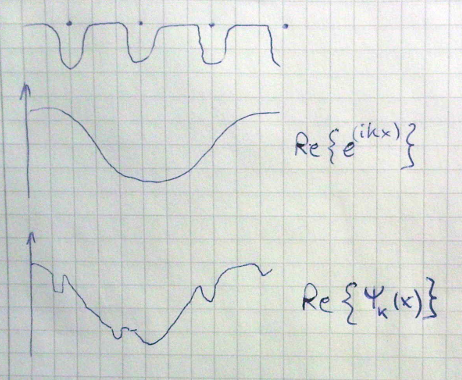
\includegraphics[width=0.75\textwidth]{kap06_35.png}
 
\begin{align}
\psi_k(\vec r+\vec R) &= \underbrace{U_k(\vec r+\vec R)e^{i\vec k\vec r}}_{\psi_{\vec r}}e^{i\vec k\vec R}
\end{align}

\[\psi_{k+G}(\vec r) \sum_G c_{k+g'-G}e^{i(\vec k+G'-G)\vec r}\]

Umbenennung \(G''=G-G'\)

\[\Rightarrow e^{i\vec k\vec r}\sum_{G''} \underbrace{c_{\vec k-\vec G''}e^{-i\vec G''\vec r}}_{U_{\vec k}(\vec r)}\]
\[\Rightarrow \psi_{\vec k+\vec a}(\vec r) = \psi_k(\vec r)\]

\[H\psi_{k+G}(\vec r) = E_{\vec k+\vec G'}\psi_{\vec k+\vec G'}(\vec r)\]
\[H\psi_{k}(\vec r) = E_{\vec k+\vec G'}\psi_{\vec k}(\vec r)\]
\[\Rightarrow E_{k+G'}=E_k\]

Lösung der SG. an der Grenze der Brillouin Zone. 

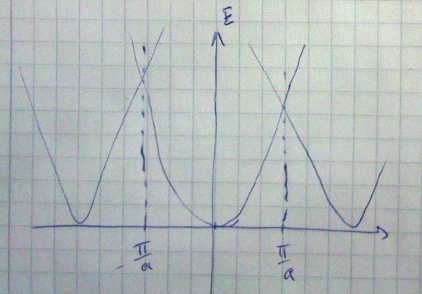
\includegraphics[width=0.75\textwidth]{kap06_36.png}

\[(E-\frac{\hbar^2}{2m}|k-G|^2 )c_{k-G}=\sum_G \tilde V_{G'}c_{k-G-G'}\]

\begin{align}
c_{k-G} &= \frac{\sum_G \tilde V_{G'}c_{k-G-G'}}{E-\frac{\hbar^2}{2m}|k-G|^2}\\
&= \frac{\sum_{G''}V_{G''-G}c_{k-G''}}{\frac{\hbar^2}{2m}(k^2-|k-G|^2)}
\end{align}

Umbenennung: \(G=G''-G\)
Nullstellen: \(k^2=|\vec k-\vec G|^2\)
Abkürzungen \(g=\frac{2\pi}{a}\); \(G=0\),\(G=g\); \(\lambda_k = \frac{\hbar^2 k^2}{2m}\)


Zwei Komponenten Näherung 

Erste Bedingung: \(\rightarrow (\lambda_k -E)c_k+\tilde V_g c_{k-g} = 0\)
zweite Bedingunge: \(\rightarrow (\lambda_{k-g} -E)c_{k-g}+\tilde V_g c_k = 0\)

Daraus resultieren Energieeigenwerte: \(E_{\pm}=\frac{1}{2}(\lambda_{k-g}+\lambda_k\pm \sqrt{(\lambda_{k-g}-\lambda_k)^2+\tilde V_g^2}\) und \(k=\frac{g}{2}\rightarrow \lambda_{k-g}=\lambda_k\)

An der Grenze der Brillouin Zone

\[ E_{\pm} = E_{\frac{g}{2}}\pm|\tilde V_g| \]

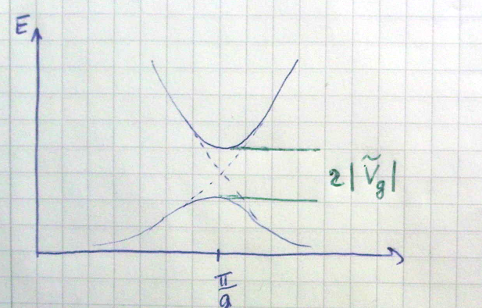
\includegraphics[width=0.75\textwidth]{kap06_37.png}

\(\frac{c_{k-G}}{c_k}=\frac{E-\lambda}{\tilde V_g}\)


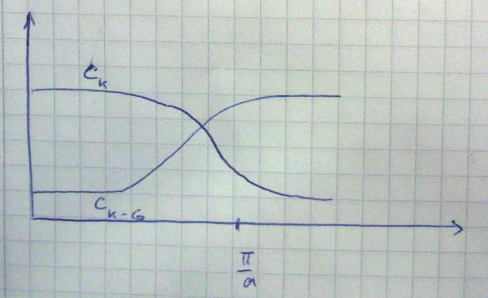
\includegraphics[width=0.75\textwidth]{kap06_38.png}



\section{Tight-binding Model}

\underline{'stark gebundene Elektronen'}


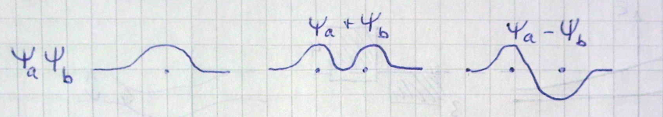
\includegraphics[width=0.75\textwidth]{kap06_39.png}

\[\rho \propto |\psi_a-\psi_b|^2\]


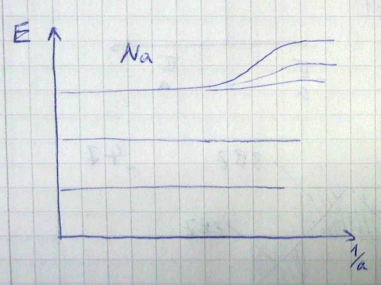
\includegraphics[width=0.75\textwidth]{kap06_40.png}
LCAO = Linear Combination of Atomic Orbitals

\[H\phi = E\phi\]
\[H= H_A+H_S\quad (m\neq n)\]
\[H = -\frac{\hbar^2}{2m}\nabla + \tilde V(\vec r - \vec R_m)\qquad R_m\equiv\text{Gittervektor}\]
\[H_S = \sum_{n\neq m}\tilde V_A(\vec r - \vec R_n)\]

Energie eigenwerte \(E_k\)

\[ E_k = \frac{\int \psi^* H\psi dV}{\int \psi^*\psi dV}\]

 µ·µ·\[\psi_{\vek k} = \sum_m a_m\phi(\vec r\cdot\vec R_m)\qquad a_m=\frac{1}{\sqrt{N}} e^{i\vec k\vec R_m}\quad N\equiv\text{Anzahl der Atome}\]


Bloch-Funktionen \(\rightarrow \) orthonormal Basis lokalisierter Zustände Wnnier-Funkitonen

\[w_m(\vec r\cdot\vec R_m) = \frac{1}{\sqrt{N}}\sum_{\vec k}e^{-i\vec k\vecR_m}\psi_k(\vec r- \vec R_m)\]
\[\psi =\frac{1}{\sqrt{N}}\sum_{\vec R_m}e^{i\vec k\vecR_m}w_m(\vec r- \vec R_m) \]
\[E_{\vec k} = \frac{1}{\underbrace{\int \phi^*\phi dV}_{=1\quad\text{Wellenfkt kaum Überlappung}}}\frac{1}{N}\sum_{m,n}e^{ik(Rm-R_n)}\int\phi^*(r-R_n)[H_A+H_S(\vec r-\vec R_m)\phi(\vec r-\vec R_m)dV]\]
\[\alpha = -\int \phi^*(r-R_m)H_s(\vec r-\vec R_m)\phi(\vec r -\vec R_m)dV \equiv\text{Energieänderung durch das Nachbarpotential}\]

\[\beta = -\int \phi^*(\vec r- \vec R_n)H_S(\vec r-\vec R_m)\phi(\vec r-\vec R_n)\equiv\text{Energieänderung durch den Überlapp der W.F.}\]

\begin{align}
E_{ki} &= E_i - \alpha_i - \sum\beta_{i,n}e^{ik(R_n-R_m}\\
&= E_i - \alpha_i2\beta_{i}(cos(k_xa)+cos(k_y a)
\end{align}

Für ein kubisch primitives Gitter \(R_m-R_n=(\pm a,00),(0\pm a,0),(0,a\pm a)\); \(\Rightarrow \) Entwickeln für kleine \(k\):

\[E_{k,i}=E_i - \alpha_i-6\beta_i+\beta_i a^2k^2\]



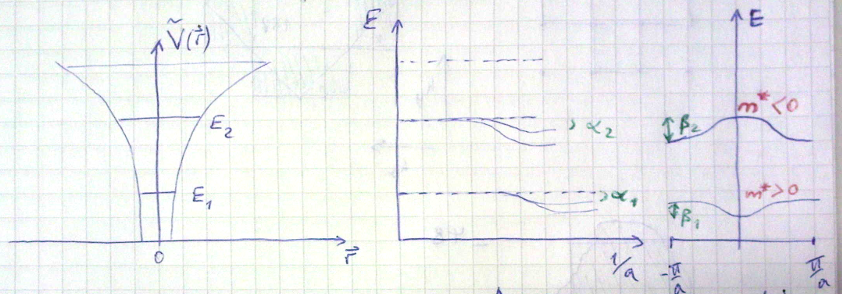
\includegraphics[width=0.75\textwidth]{kap06_41.png}

\[E_i=\frac{\hbar^2k^2}{2m}\Rightarrow m^*_i=\frac{\hbar^2}{2\beta_ia^2}\]

Energiedispersionspektrum \(E_i(k)\)

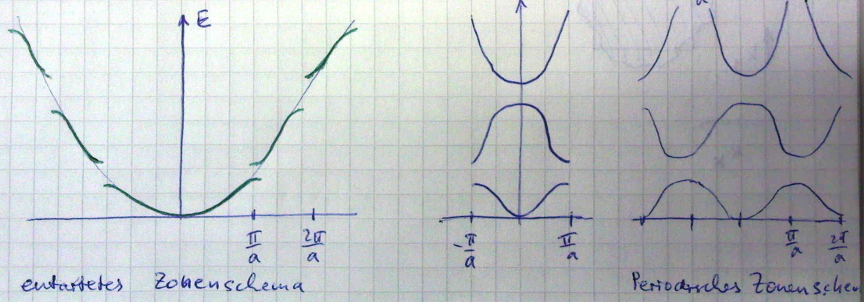
\includegraphics[width=0.75\textwidth]{kap06_42.png}


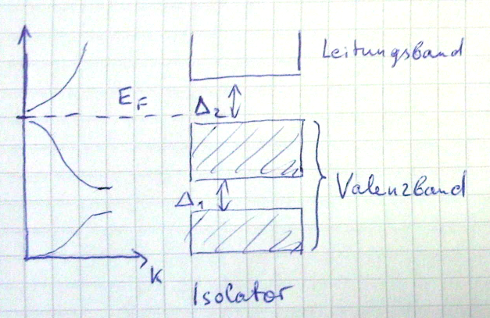
\includegraphics[width=0.75\textwidth]{kap06_43.png}

Isolator, \(\rho = 10^7-10^{14}\Omega m\); \(E_F = \frac{\hbar^2}{2m}(3\pi^2 n_e)^{2/3}\)

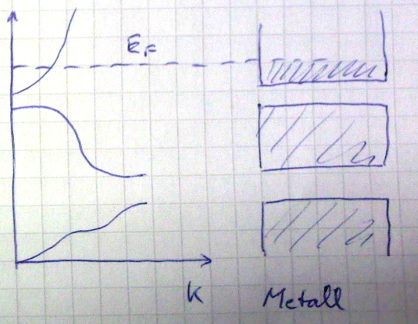
\includegraphics[width=0.75\textwidth]{kap06_44.png}

Metall: \(\rho = 10^{-4}-10^{-8}\Omega m\); 


2D-Gitter \(\rightarrow \) verschiedene Kristallrichtung


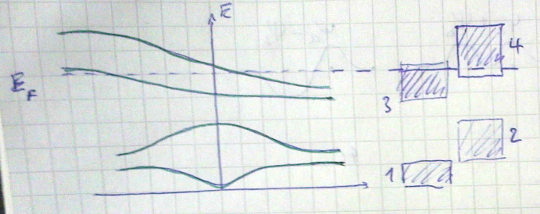
\includegraphics[width=0.75\textwidth]{kap06_45.png}


Halbmetalle As, Sb(Antimon), Bi 

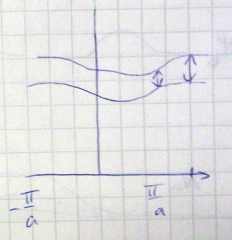
\includegraphics[width=0.75\textwidth]{kap06_46.png}


Brillion-Zonen und Fermi Flächen (2D BZ)

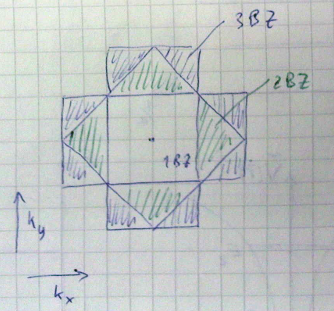
\includegraphics[width=0.75\textwidth]{kap06_47.png}

an der zonengrenze (stehende Wellen)
\[\frac{\partial\omega}{\partial k}=\frac{1}{\hbar}\vec \nabla E_\bot =0\]
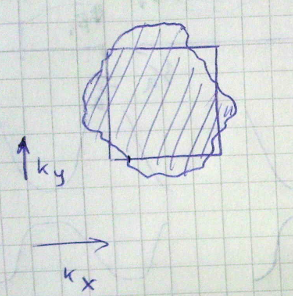
\includegraphics[width=0.75\textwidth]{kap06_48.png}




\end{document}
